\documentclass[logo,reportComp]{thesis}
\usepackage[python,javascript,linenum]{mypackage}
\title{数据库系统期末大作业}
\subtitle{AIDO项目设计报告}
\school{数据科学与计算机学院}
\author{陈鸿峥\qquad 刘学海\qquad 刘佳荣\\17341015\qquad 17341111\qquad 17341109}
\classname{17大数据与人工智能}
\stunum{}
\headercontext{数据库系统期末大作业}

\begin{document}

\maketitle

\section{概览}
本次项目我们开发了一套人工智能日程管理系统,实现智能对话、日程管理、语音输入识别与输出等多项功能,效果概览图可见图\ref{fig:overview}。
\begin{figure}[H]
\centering
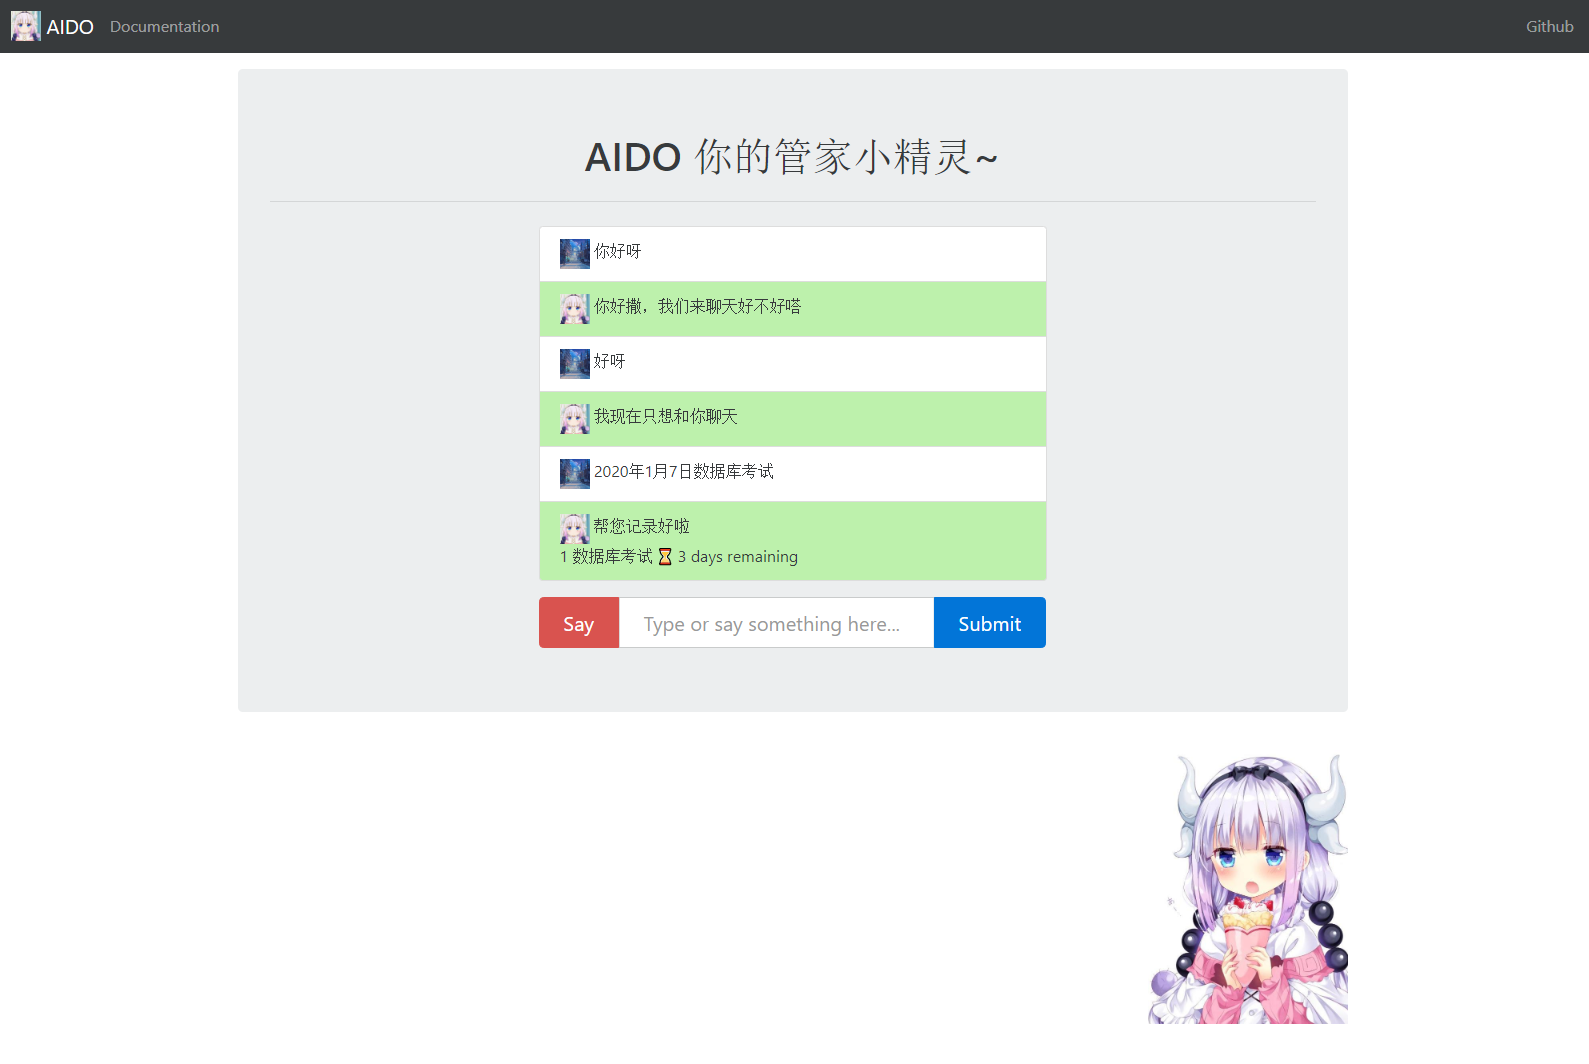
\includegraphics[width=\linewidth]{fig/overview.png}
\caption{AIDO:你的智能小管家}
\label{fig:overview}
\end{figure}

\textcolor{red}{本项目已经部署上腾讯云服务器,可通过\url{http://193.112.60.186:8056/}进行访问。}
% \textcolor{red}{本项目已经部署上腾讯云服务器,可通过\url{http://xxx.xxx.xx.xxx:8056/}进行访问。}

本项目的所有源代码公开于\url{https://github.com/reacherhai/AIDO},或可查看本项目下的\verb'source'文件夹。
\textbf{更多细节可见}\verb'document.pdf'\textbf{,其中包含了市场调查、竞品分析、产品特点与使用说明等。}
如需自己安装服务器并运行,请查看\verb'README.md'进行部署。
下面将会简要叙述本项目的要求及设计动机。

\subsection{项目要求}
本项目需要我们设计一个数据库应用,采用客户端/服务器的结构,具体要求如下:
\begin{itemize}
\item 有完整的前后端架构(前端界面+后台数据库)
\item 内容有实际意义且完整
\item 支持对数据的增删改查操作
\end{itemize}

\subsection{设计动机}
我们小组做这个项目最初的动机来源于前半学期实验中做的TodoList。TodoList的作用类似于实际生活中的备忘录或是手账,用户可以在TodoList中记录自己未来要做的事情,并且可以修改记录,或者是对记录进行标记(比如打上已经完成的标记)。通过使用这类工具,用户可以有效地管理未来的事务。

我们认为,现在的生活中,每个人都面临着繁琐的日常事务。就以学生来说,各门课都会布置作业,作业都有各自的DDL,如果没有进行有效的管理,会导致规划时间不合理或是忘记作业等问题。所以我们认为管理个人未来事务是一种需求,我们可以针对这种需求去做一个项目。

虽然TodoList可以达成管理个人事务这一目的,但我们认为仅仅如此是不够的,TodoList存在一些问题。TodoList中每一项记录的添加、删除、修改都要通过打字或多次操作实现,这在一定程度上增加了使用的难度,从而降低用户使用TodoList的积极性,而这种类似于备忘录的应用如果更少地被使用,它的作用是要打折扣的。同时,TodoList的功能单一,只有备忘录这一功能,用户使用的积极性也比较低,这会带来与前一点相同的影响。

所以为了解决上述的两个问题,我们小组旨在设计一个类似于微软小冰或是小黄鸡的,能协助管理个人事务的智能机器人AIDO。
而这里的名称AIDO借用了偶像(idol)的谐音,方便易记,希望能够真正成为用户心中的偶像与朋友。

\textbf{目前该项目主要部署在web端,用户不需要进行下载,更加方便应用的使用与传播。
用户可直接像平时聊天一样进行键盘输入或语音输入,没有任何使用或安装门槛。}

\subsection{技术栈}
\begin{flushleft}
\begin{tabular}{ll}
\textbf{开发语言} &\qquad JavaScript\ /\ HTML\ /\ CSS\ /\ Python\ /\ SQLite\\
\textbf{浏览器环境} &\qquad Chrome\ /\ Firefox\ /\ Safari\\
\textbf{第三方库}  &\qquad jQuery\ /\ Bootstrap
\end{tabular}
\end{flushleft}

\subsection{项目分工}
整个项目主要分为两个部分,前期准备规划以及代码的实现与测试。

前期规划阶段没有十分明显的分工,主要是三人针对TodoList现有的问题进行分析,并进行调研,调查市场上类似产品,分析自己做的东西是否有意义。之后,进行规划,明确需要实现的需求,包括智能机器人以及事务管理两部分。再然后,进行工作的分配,并进行准备。

代码的实现与测试阶段的分工如下。

\textbf{陈鸿峥:}
\begin{itemize}
\item 前端页面的搭建与整合
\item 页面的设计与美化
\end{itemize}

\textbf{刘学海:}
\begin{itemize}
\item 产品功能设计
\item 后端接口的设计与实现
\item 数据库设计
\end{itemize}

\textbf{刘佳荣:}
\begin{itemize}
\item 明确需求与实现,编写文档报告
\item 对应用进行运行测试,反馈前后端
\end{itemize}

\section{项目特点}

AIDO的主要设计目的是打造一个帮助管理日常事务的智能管家,让用户能便捷、有效地管理日常事务,并提供友好的交互界面。其主要特征有:
\begin{itemize}
\item \textbf{聊天交互功能:}AIDO模仿了现有的小黄鸡等应用,实现了用户与机器人之前的交互功能。
\begin{figure}[H]
\centering
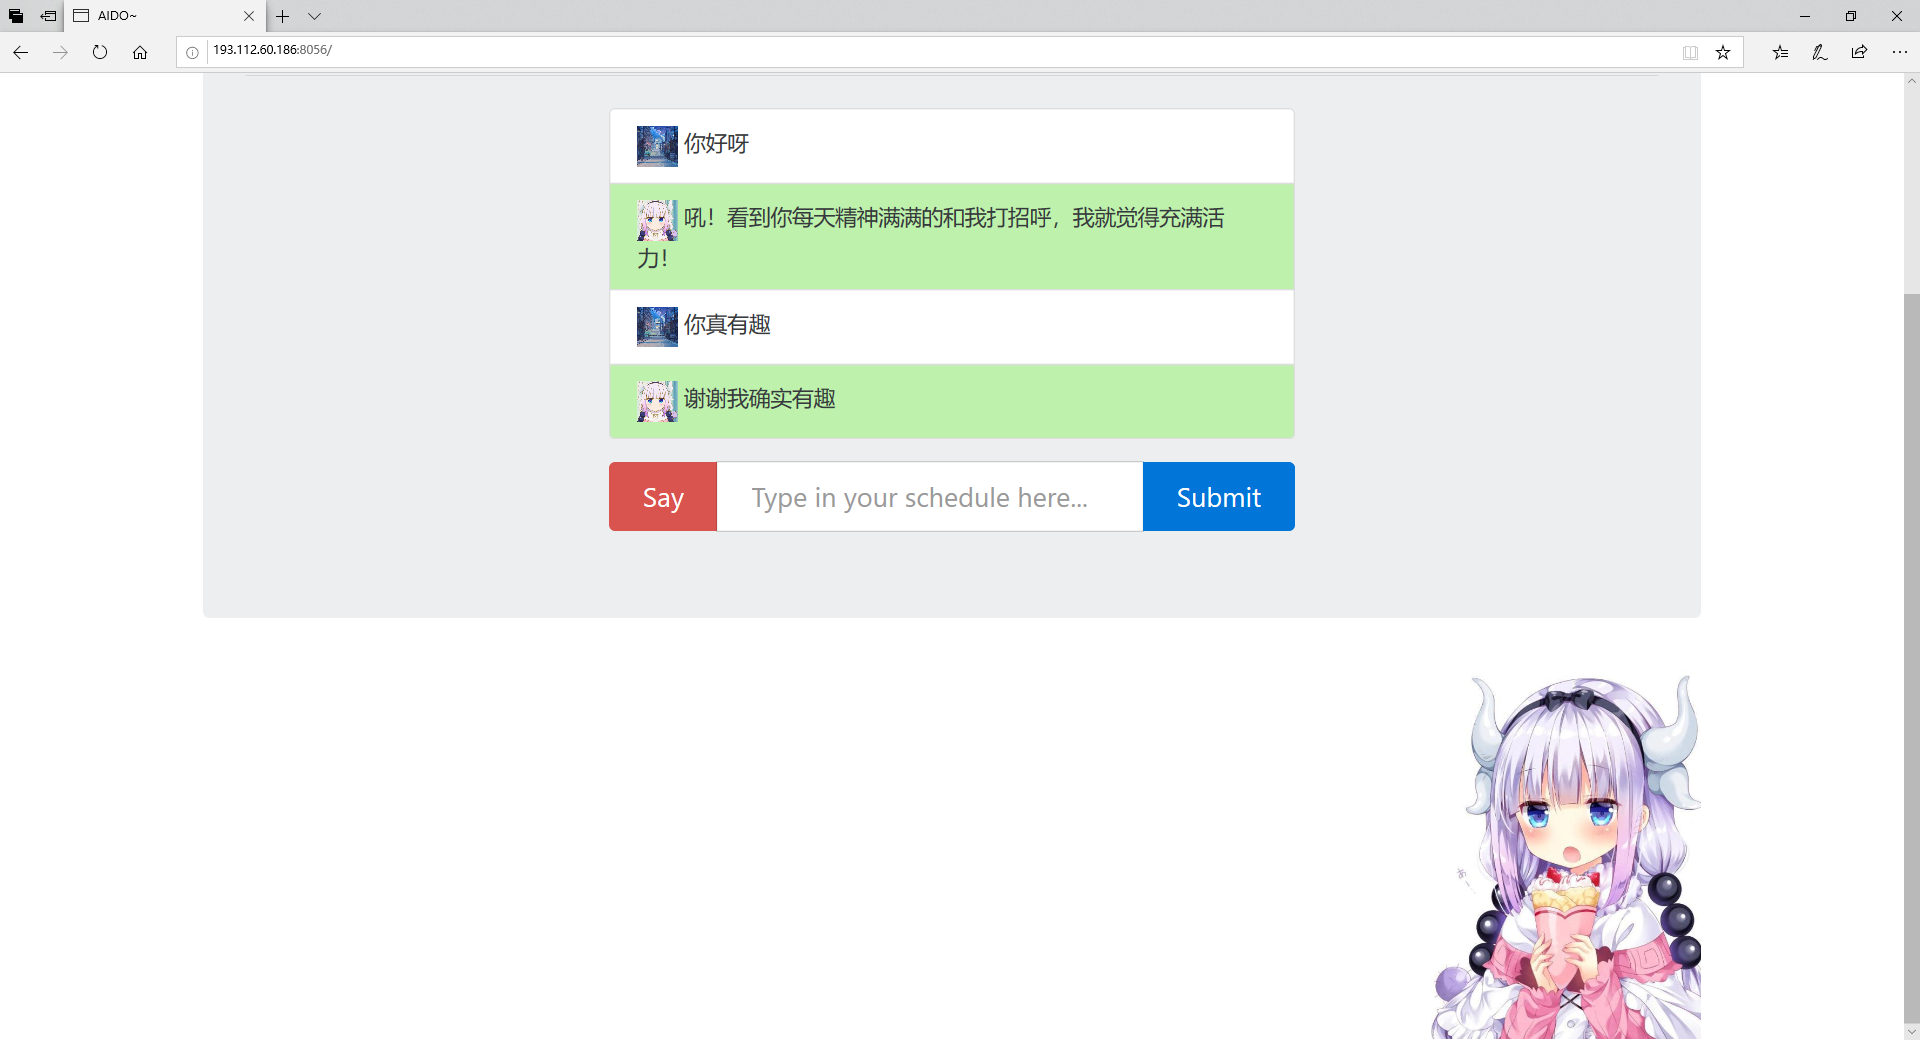
\includegraphics[width=\linewidth]{fig/chatting}
\end{figure}

我们的机器人支持\textbf{语音输入},按住say按钮就可以进行录音。录音文件会保存到本地。同时,机器人也会根据语音进行相应的回答(打开音响可以听到\textbf{语音反馈})。用户可以通过与智能机器人交流,达到近似于与真人进行交流的体验。与此同时,下面的一系列功能都支持语音输入和语音输出,最大程度释放用户的双手。
\item \textbf{日常查询功能:}AIDO可以根据用户输入的信息,解释相关概念。
\begin{figure}[H]
\centering
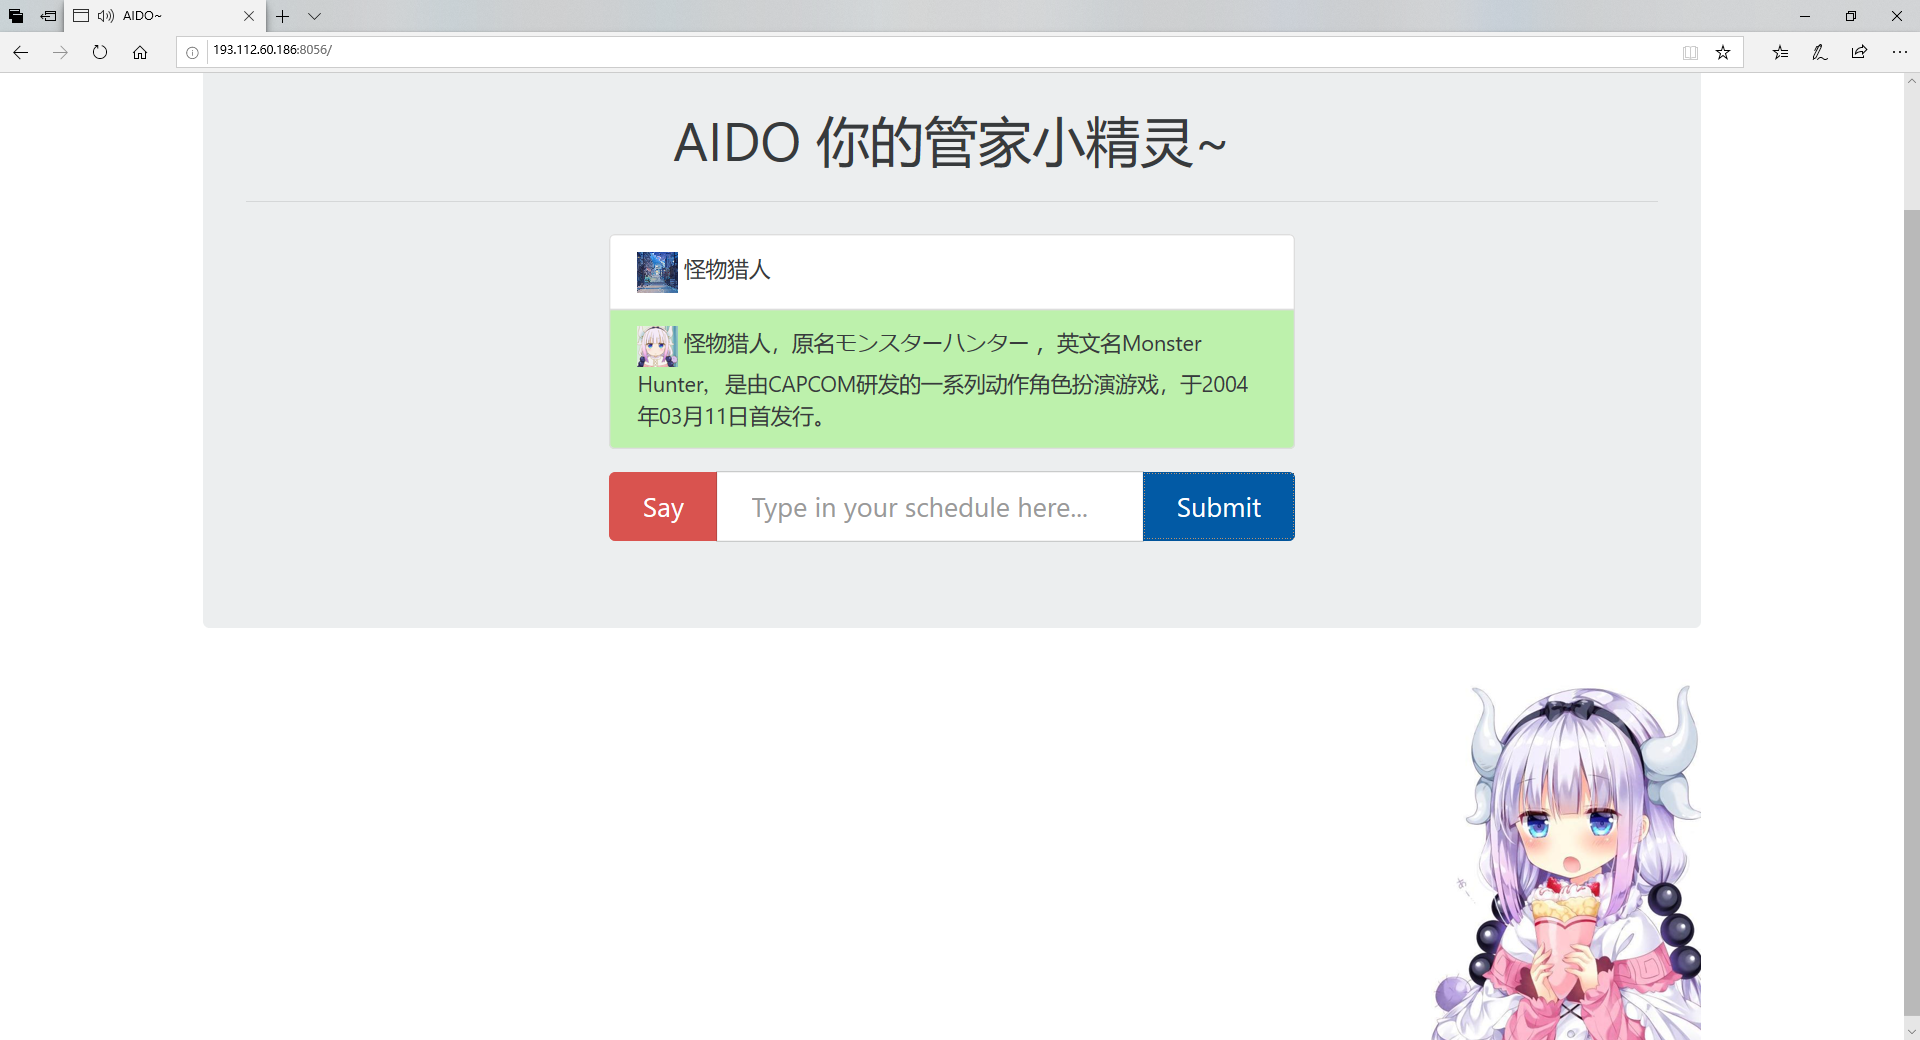
\includegraphics[width=\linewidth]{fig/wiki}
\end{figure}

用户可以输入想要了解的人物/事务,机器人就会为用户提供对应概念的解释,此处机器人提供的解释主要来源于百度百科。
\item \textbf{添加任务功能:}AIDO可以实现帮用户添加任务事项的功能。
\begin{figure}[H]
\centering
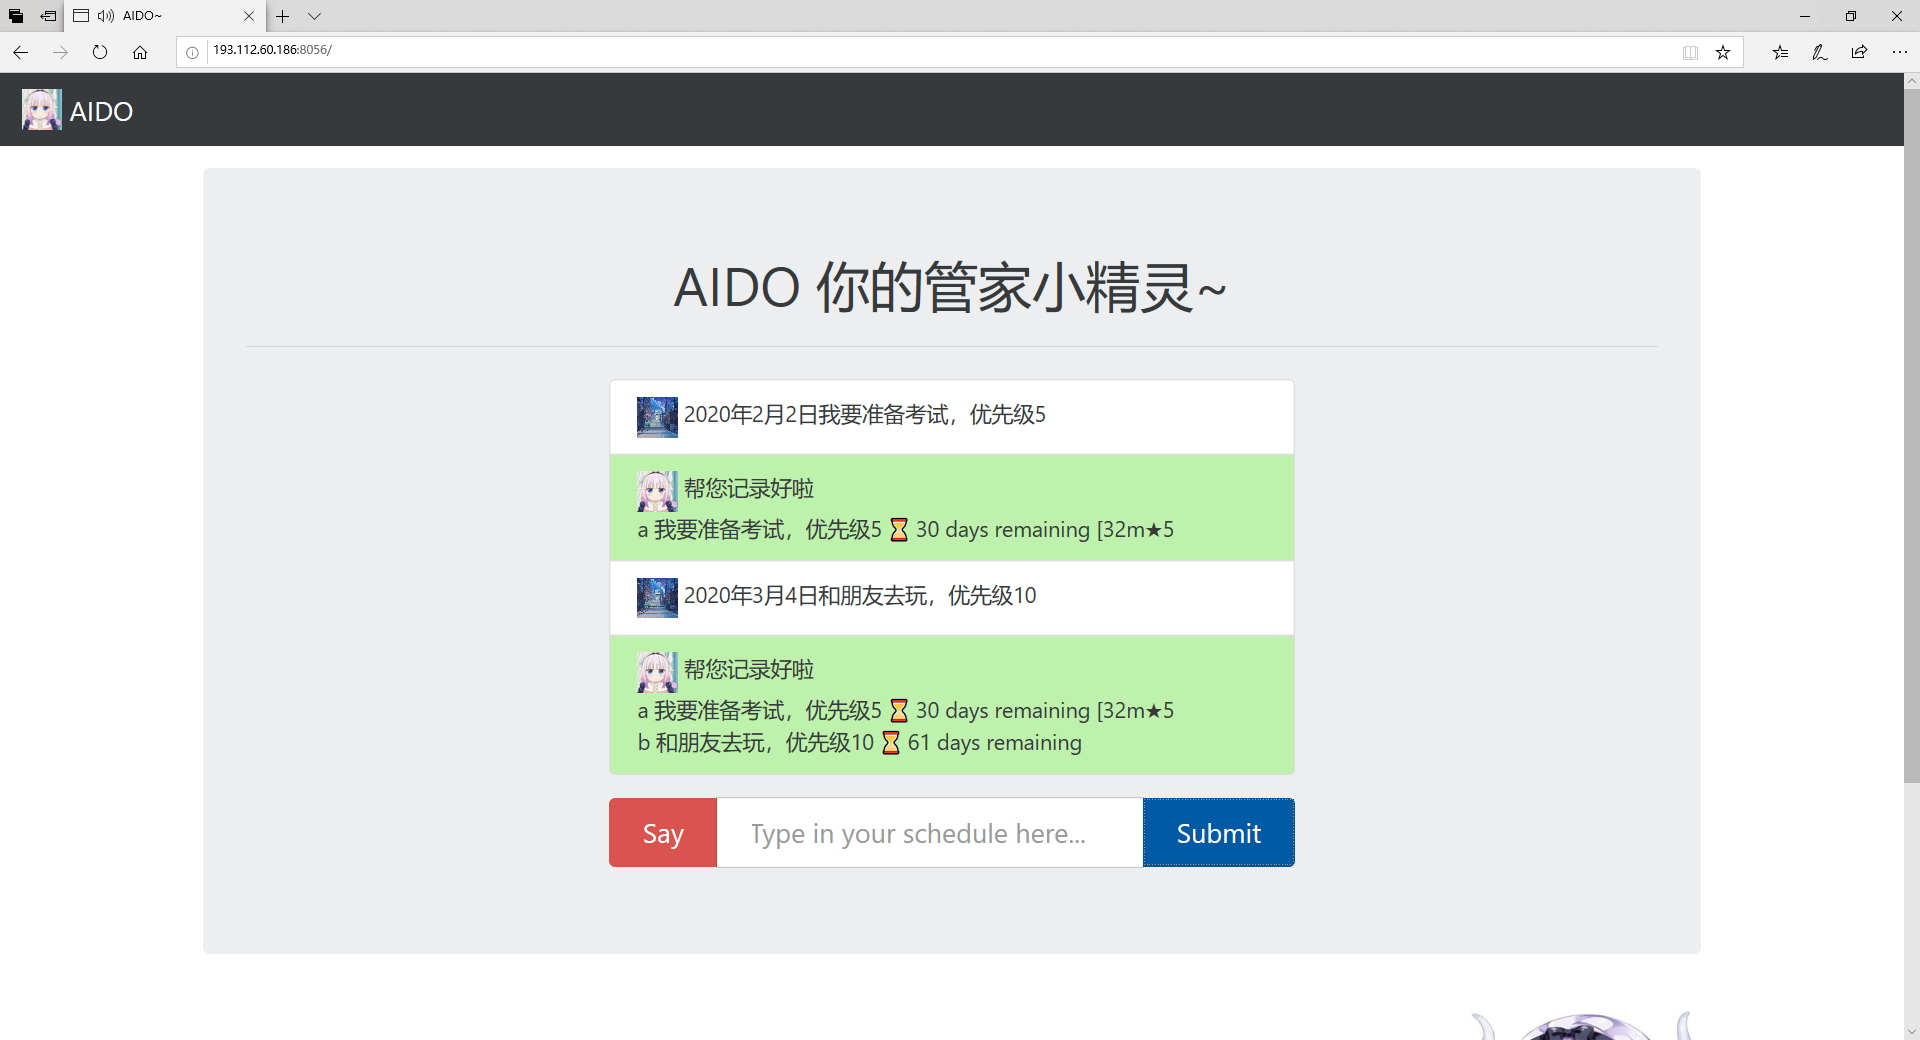
\includegraphics[width=\linewidth]{fig/add_task}
\end{figure}

用户输入日期(****年*月*日)+任务,机器人将帮用户录入TodoList,并自动计算距离deadline的时间。此外,支持给任务添加优先级。在任务中添加“优先级”+数字,奇迹人将自动检测任务的优先级并将高优先级的任务排在前面。
\item \textbf{删除任务功能:}AIDO可以实现帮助用户删除任务事项的功能。
\begin{figure}[H]
\centering
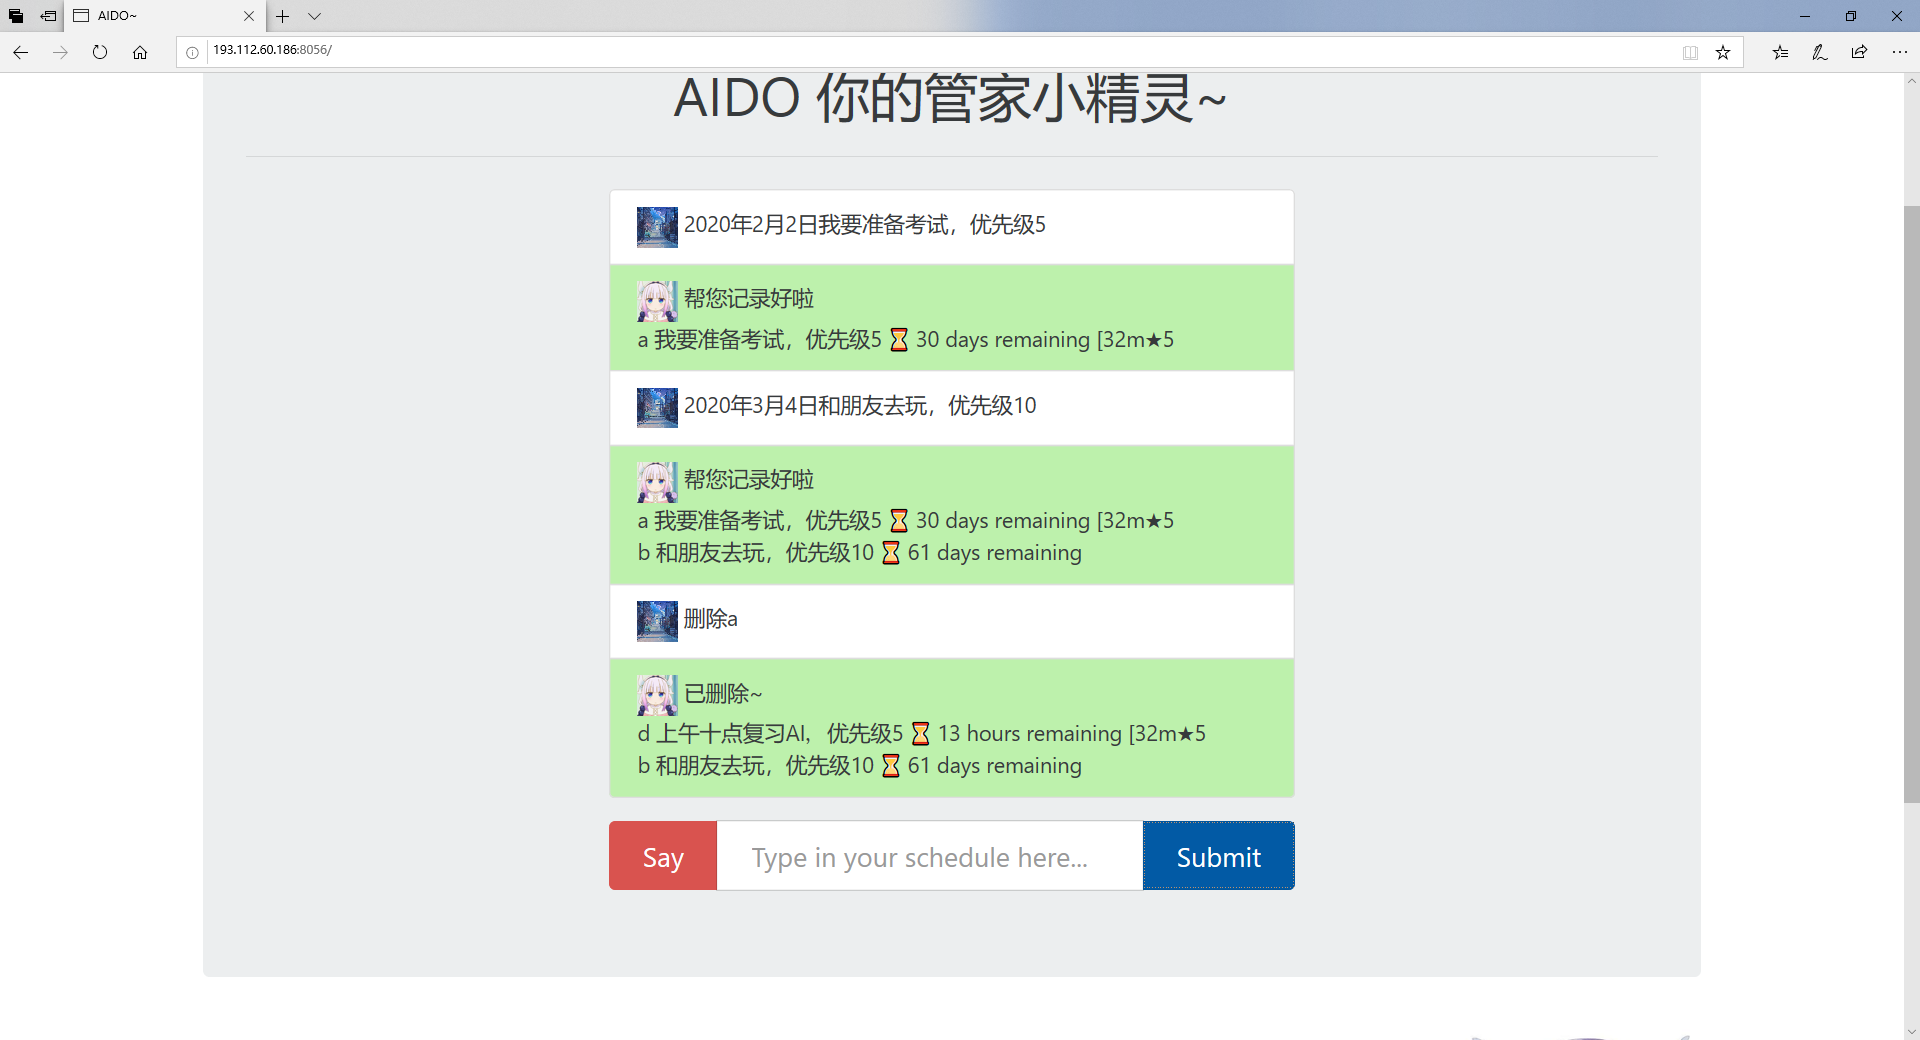
\includegraphics[width=\linewidth]{fig/del_task}
\end{figure}

通过输入“删除”+任务对应的字母/数字,机器人就可以帮助用户删除对应的任务。
\item \textbf{查看待办事项功能:}AIDO允许用户查询当前剩余的待办事项。
\begin{figure}[H]
\centering
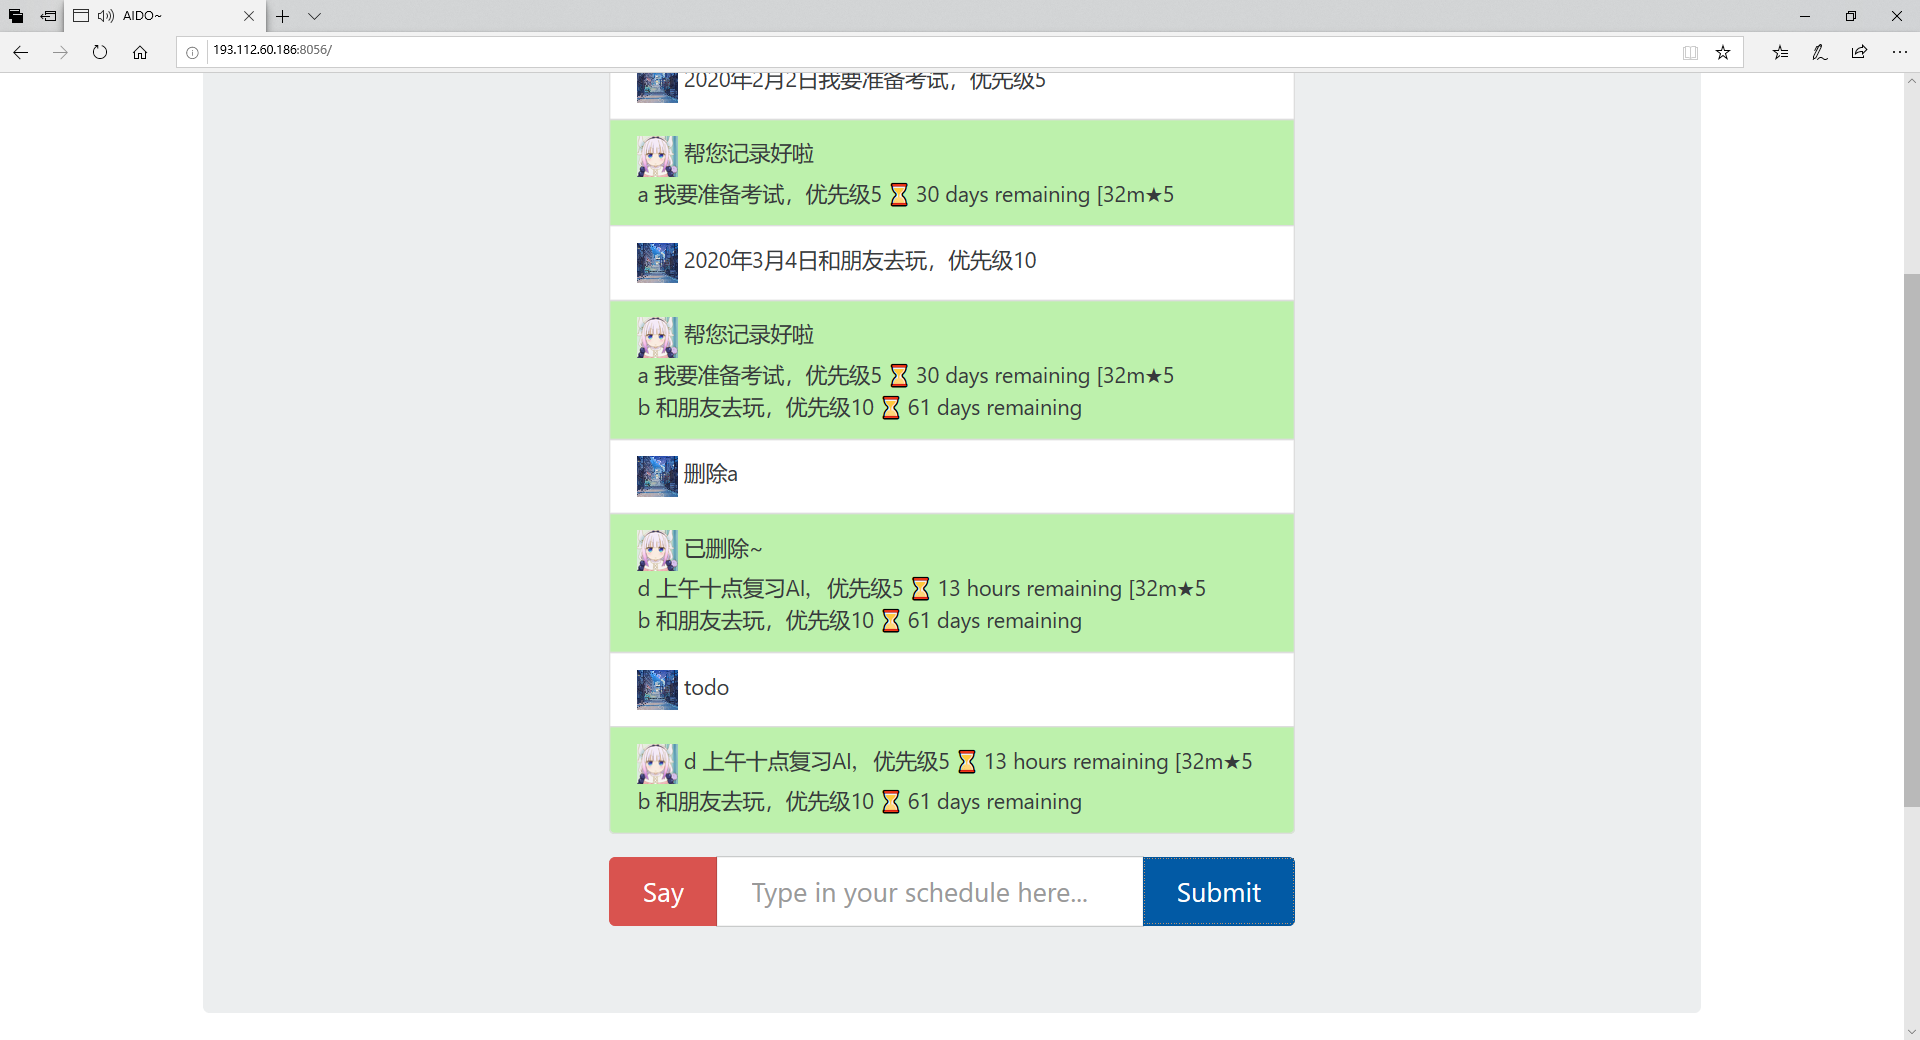
\includegraphics[width=\linewidth]{fig/ask_task}
\end{figure}

通过输入“todo”,用户可以查看现有的所有待办事项的详细信息。
\end{itemize}

我们的项目主要包含了以上功能,可以说,AIDO包含了TodoList的核心功能,但同时加入了智能机器人这一辅助工具,使个人事务的管理可以统一使用语音输入这一手段进行管理,增加了效率和方便性,又使得应用场景更丰富,机器人可以协助解决除事务管理外的其它问题。同时,AIDO也提供了更为美观、友好的交互界面,给用户带来更好的体验。

\section{ER图与关系模式设计}
\subsection{ER图}

本项目设计的ER图如图\ref{fig:er}所示。
\begin{figure}[H]
\centering
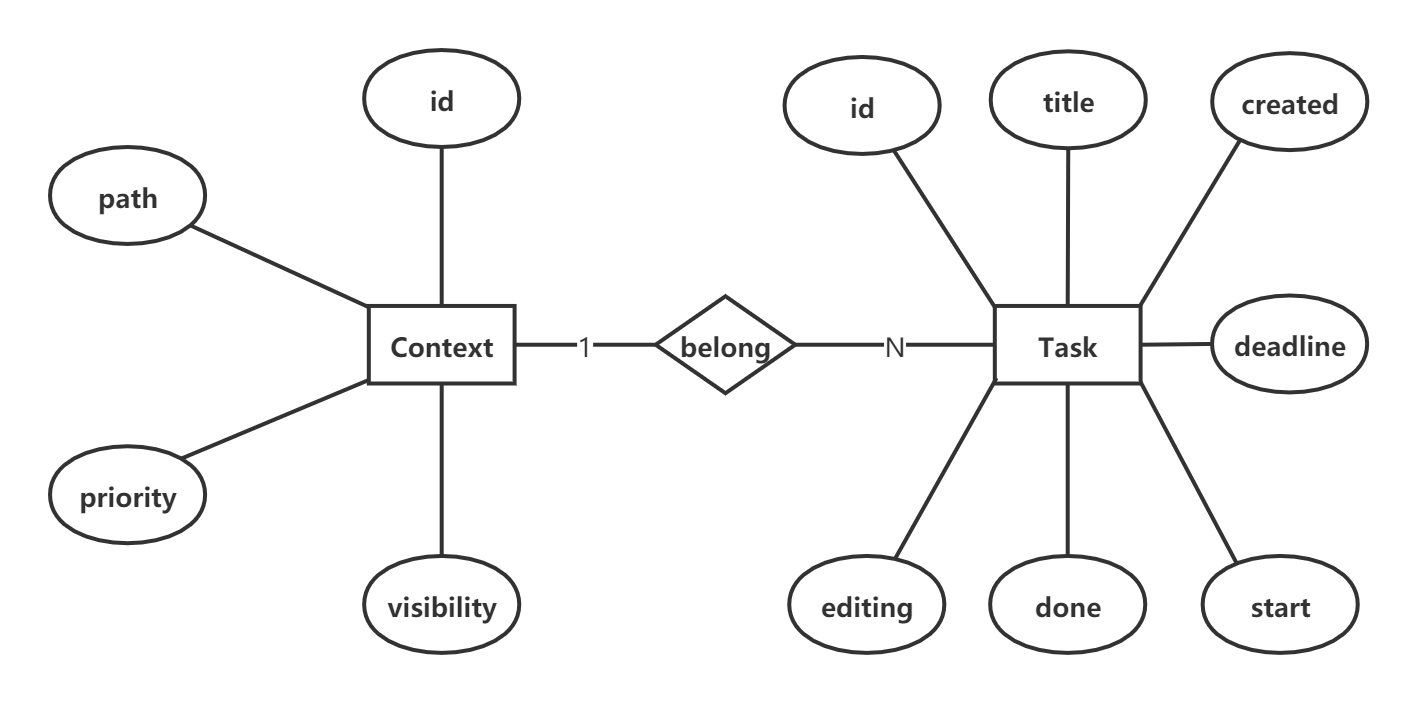
\includegraphics[width=\linewidth]{fig/er_design}
\caption{项目设计E-R图}
\label{fig:er}
\end{figure}

\subsection{关系模式与建表语句}

根据以上ER图,我们可以建立以下关系模式:
\begin{itemize}
\item \textbf{Task(\uline{id}, title, created, deadline, start, priority, done, \uwave{context}, content, editing)}
\begin{lstlisting}[language=SQL]
CREATE TABLE `Task` (
	`id`	INTEGER NOT NULL PRIMARY KEY AUTOINCREMENT UNIQUE,
	`title`	TEXT NOT NULL,
	`created`	TEXT NOT NULL DEFAULT (datetime('now')),
	`deadline`	TEXT,
	`start`	TEXT NOT NULL DEFAULT (datetime('now')),
	`priority`	INTEGER NOT NULL DEFAULT 1,
	`done`	TEXT,
	`context`	INTEGER NOT NULL REFERENCES Context(id) ON DELETE CASCADE
);
CREATE INDEX `DoneIndex` ON `Task` (`done`);
CREATE INDEX `DateCreatedIndex` ON `Task` (`created`);
ALTER TABLE Task ADD COLUMN `content` TEXT;
ALTER TABLE Task ADD COLUMN `editing` INTEGER NOT NULL DEFAULT 0;
\end{lstlisting}
\item \textbf{Context(\uline{id}, path, priority, visibility)}
\begin{lstlisting}[language=SQL]
CREATE TABLE `Context` (
	`id`	INTEGER NOT NULL PRIMARY KEY AUTOINCREMENT UNIQUE,
	`path`	TEXT NOT NULL UNIQUE,
	`priority`	INTEGER NOT NULL DEFAULT 1,
	`visibility`	TEXT NOT NULL DEFAULT 'normal'
);
INSERT INTO `Context` (path) VALUES ('');
CREATE INDEX `PathIndex` ON `Context` (`path` ASC);
\end{lstlisting}
\end{itemize}

\section{设计细节}

本节主要介绍各个部分的设计细节,包括其中涉及的代码细节与SQL语句。

\subsection{TodoList}
TodoList的实现主要包含了四个模块,添加任务,删除任务, 修改任务以及查询任务。
\subsubsection{添加任务}

TodoList中有任务的添加,以及环境(context)的添加。
\begin{itemize}
\item 任务添加
\begin{lstlisting}[language=SQL]
INSERT INTO Task (title, content, context {})
VALUES (?, ?, ? {})
\end{lstlisting}
\item 环境添加
\begin{lstlisting}[language=SQL]
INSERT INTO Context (path)
VALUES (?)
\end{lstlisting}
\item 将一个路径中的任务复制到另一路径
\begin{lstlisting}[language=SQL]
UPDATE Task
SET context = ?
WHERE context = (
	SELECT id FROM Context
	WHERE path = ?
)
\end{lstlisting}
\end{itemize}

\subsubsection{删除任务}

TodoList中有对数据的删除操作,其中包括了删除任务,删除环境,以及删除满足某些要求的任务。
\begin{itemize}
\item 删除特定id的任务
\begin{lstlisting}[language=SQL]
DELETE FROM Task
WHERE id = ?
\end{lstlisting}
\item 删除特定路径的环境
\begin{lstlisting}[language=SQL]
DELETE FROM Context
WHERE path LIKE ?
\end{lstlisting}
\item 删除某时刻前产生,并且已完成的任务
\begin{lstlisting}[language=SQL]
DELETE FROM Task
WHERE done IS NOT NULL
AND created < ?
\end{lstlisting}
\end{itemize}

\subsubsection{修改任务}

TodoList中有对任务的修改操作,其中主要是修改任务内容,或是更改任务的标记内容(完成标记以及编辑标记)。
\begin{itemize}
\item 修改特定id的任务
\begin{lstlisting}[language=SQL]
UPDATE Task SET {}
WHERE id = ?
\end{lstlisting}
\item 标注特定id的任务状态为完成
\begin{lstlisting}[language=SQL]
UPDATE Task SET done = datetime('now')
WHERE id = ?
AND done IS NULL
\end{lstlisting}
\item 标记特定未处于编辑的任务为编辑状态
\begin{lstlisting}[language=SQL]
UPDATE Task
SET editing = 1
WHERE id = ?
  AND editing = 0
\end{lstlisting}
\item 释放某任务的编辑状态
\begin{lstlisting}[language=SQL]
UPDATE Task
SET editing = 0
WHERE id = ?
\end{lstlisting}
\end{itemize}

\subsubsection{查询任务}

TodoList中有如下的各种查询操作。
\begin{itemize}
\item 查询特定id的任务
\begin{lstlisting}[language=SQL]
SELECT t.*, c.path as ctx_path
FROM Task t JOIN Context c
ON t.context = c.id
WHERE t.id = ?
\end{lstlisting}
\item 根据路径查询环境id
\begin{lstlisting}[language=SQL]
SELECT id FROM Context
WHERE path = ?
\end{lstlisting}
\item 查询特定路径的环境是否存在
\begin{lstlisting}[language=SQL]
SELECT 1 FROM Context
WHERE path = ?
\end{lstlisting}
\item 查询特定路径环境包含的任务数和子环境数
\begin{lstlisting}[language=SQL]
SELECT COUNT(t.id)
FROM Task t
JOIN Context c
ON t.context = c.id
WHERE t.done IS NULL
AND c.path = ?
UNION ALL
SELECT COUNT(id)
FROM Context
WHERE path LIKE ?
\end{lstlisting}
\item 查询特定路径下的所有任务(这些任务直接在该目录下,不在子目录):
\begin{lstlisting}[language=SQL]
SELECT t.*, c.path as ctx_path
FROM Task t JOIN Context c
ON t.context = c.id
WHERE c.path = ?
  AND t.done IS NULL
  AND (c.path = ? OR c.visibility = 'normal')
  AND (datetime('now')) >= datetime(t.start)
ORDER BY
  priority DESC,
  COALESCE(
      julianday(deadline),
      julianday('9999-12-31 23:59:59')
    ) - julianday('now') ASC,
  created ASC
\end{lstlisting}
\item 查询最大的任务id
\begin{lstlisting}[language=SQL]
SELECT MAX(id)
FROM Task
\end{lstlisting}
\item 查询特定路径下特定标题的任务
\begin{lstlisting}[language=SQL]
SELECT t.*, c.path as ctx_path
FROM Task t JOIN Context c
ON t.context = c.id
WHERE t.title LIKE ?
  AND c.path LIKE ?
\end{lstlisting}
\end{itemize}

\subsection{对话机器人}
我们使用了一个类Chatbot来封装机器人的所有功能。机器人的核心模块使用面向对象的接口形式进行封装。
\begin{itemize}
    \item \textbf{语音输入}\\
    语音输入部分,机器人获取用户的输入并将录音文件保存到本地的media/voice\_ss.mp3。实现类recorder如下:
\begin{lstlisting}
from pyaudio import PyAudio, paInt16
import numpy as np
import wave

class Recorder:
    NUM_SAMPLES = 2000      # `py audio内置缓冲大小'
    SAMPLING_RATE = 16000    # `取样频率'
    LEVEL = 500         # `声音保存的阈值'
    COUNT_NUM = 20      # `NUM\_SAMPLES个取样之内出现COUNT\_NUM个大于LEVEL的取样则记录声音'
    SAVE_LENGTH = 8         # `声音记录的最小长度:SAVE\_LENGTH * NUM\_SAMPLES 个取样'
    TIME_COUNT = 20     # `录音时间,单位s'

    Voice_String = []

    def savewav(self, filename):
        wf = wave.open(filename, 'wb')
        wf.setnchannels(1)
        wf.setsampwidth(2)
        wf.setframerate(self.SAMPLING_RATE)
        wf.writeframes(np.array(self.Voice_String).tostring())
        # wf.writeframes(self.Voice_String.decode())
        wf.close()

    def recorder(self):
        pa = PyAudio()
        stream = pa.open(format=paInt16, channels=1, rate=self.SAMPLING_RATE, input=True,
                         frames_per_buffer=self.NUM_SAMPLES)
        save_count = 0
        save_buffer = []
        time_count = self.TIME_COUNT

        while True:
            time_count -= 1
            # print time_count
            # `读入NUM\_SAMPLES个取样'
            string_audio_data = stream.read(self.NUM_SAMPLES)
            # `将读入的数据转换为数组'
            audio_data = np.fromstring(string_audio_data, dtype=np.short)
            # `计算大于LEVEL的取样的个数'
            large_sample_count = np.sum(audio_data > self.LEVEL)
            print(np.max(audio_data))
            # `如果个数大于COUNT\_NUM,则至少保存SAVE\_LENGTH个块'
            if large_sample_count > self.COUNT_NUM:
                save_count = self.SAVE_LENGTH
            else:
                save_count -= 1

            if save_count < 0:
                save_count = 0

            if save_count > 0:
                # `将要保存的数据存放到save\_buffer中'
                # print  save_count > 0 and time_count >0
                save_buffer.append(string_audio_data)
            else:
                # print save_buffer
                # `将save\_buffer中的数据写入WAV文件,WAV文件的文件名是保存的时刻'
                # print "debug"
                if len(save_buffer) > 0:
                    self.Voice_String = save_buffer
                    save_buffer = []
                    print("Recode a piece of voice successfully!")
                    return True
            if time_count == 0:
                if len(save_buffer) > 0:
                    self.Voice_String = save_buffer
                    save_buffer = []
                    print("Recode a piece of voice successfully!")
                    return True
                else:
                    return False

    def recording(self,filename):
        self.recorder()
        self.savewav(filename)
\end{lstlisting}
    
    \item \textbf{Chatbot}\\
    自动聊天部分,我们使用事先准备好的语料库对机器人进行训练。
    其中,语料库来自于百度百科、百度贴吧、微博等,语料库的详细信息请阅\url{https://github.com/codemayq/chinese\_chatbot\_corpus}。\\
    
    训练成功后,调用机器人的\verb'get_response()'接口获取自动对话信息。
    Chatbot机器人实现了下述5项功能。
    \begin{itemize}
        \item \verb'voice2text'\\
        将用户的语音输入转化成机器人可以理解的文本。
\begin{lstlisting}
    def voice2text(self):
        # `获取access\_token'
        token = getToken()
        data = {}
        data['format'] = 'wav'
        data['rate'] = 16000
        data['channel'] = 1
        data['cuid'] = str(random.randrange(123456, 999999))
        data['token'] = token
        wav_fp = open(self.voice_url, 'rb')
        voice_data = wav_fp.read()
        data['len'] = len(voice_data)
        data['speech'] = base64.b64encode(voice_data).decode('utf-8')
        post_data = json.dumps(data)
        # `语音识别的api url'
        upvoice_url = 'http://vop.baidu.com/server_api'
        r_data = urllib.request.urlopen(upvoice_url, data=bytes(post_data, encoding="utf-8"),timeout=10).read()
        logger.info(json.loads(r_data))
        err = json.loads(r_data)['err_no']
        if err == 0:
            return json.loads(r_data)['result'][0]
        else:
            return json.loads(r_data)['err_msg']
\end{lstlisting}
        
        \item \verb'get_response'\\
        根据获取的用户输入文本,调用对话接口和TodoList接口综合得到回复。如果用户输入符合TodoList的接口需求,则调用TodoList接口管理用户的待办事项。否则,调用对话接口获取机器人的聊天回复。
\begin{lstlisting}
    def get_response(self,text,voice_flag=False):
        prefix = "  "
        if not voice_flag:
            data = self.get_data(text)
        else:
            self.recording()
            text = self.voice2text()
            data = self.get_data(text)

        if (text == "todo"):
            output = os.popen("todo").read()
            output = deal_control_char(output)
            logger.info(output)
            if output != "":
                return prefix + "`您的待办事项有以下这些哦:'\n" + output
            else:
                return prefix + "`您没有待办事项哦'~"

        if(text == "setup"):
            os.popen("rm -rf ~/.toduh")
            return prefix + "`已为您清除所有任务'"

        if (grabdate(text)):
            command = getcommand(text)
            # return output
            try:
                output = os.popen(command).read()
            except:
                return prefix + "`添加的事项输入有问题哦'"

            output = os.popen("todo").read()
            output = deal_control_char(output)
            logger.info(output)
            return prefix + "`帮您记录好啦'\n" + output
        if (grabdel(text)):
            command = getdel(text)
            try:
                output = os.popen(command).read()
            except:
                return prefix + "`┗|`O′|┛ 嗷~~删除的信息不存在,请输入正确的删除信息(删除+数字/字母)'"
            output = os.popen("todo").read()
            output = deal_control_char(output)
            logger.info(output)
            return prefix + "`已删除~'\n" + output

        data = self.get_data(text)
        url = 'https://api.ownthink.com/bot'  # `API接口'
        try:
            response = requests.post(url=url, data=data, headers=headers,timeout=10)
            response.encoding = 'utf-8'
            result = response.json()
            answer = result['data']['info']['text']
        except:
            answer = "`LoL 小思有点忙'..."
        logger.info("Q: {}".format(text)) # used for logging
        logger.info("A: {}".format(answer))
        return prefix + answer
\end{lstlisting}
        
        \item \verb'text2voice'\\
        将机器人所返回的信息转化成语音文件,用于后续在交互界面播放。
\begin{lstlisting}
    def text2voice(self,answer):
        # `获取access\_token'
        logger.info("text2voice")
        token = getToken()
        get_url = baidu_api_url2 % (urllib.parse.quote(answer), "test", token)
        voice_data = urllib.request.urlopen(get_url).read()
        voice_fp = open(self.voice_url, 'wb+')
        voice_fp.write(voice_data)
        voice_fp.close()
        logger.info("Done writing audio file!")
        return
\end{lstlisting}
        
    \end{itemize}
\end{itemize}


\subsection{交互界面}
本次项目的前端采用Python的Django进行搭建,之所以选择Django是因为项目的后端都选择Python进行编写,而Django能够很好地跟后端进行交互,并且只需较小工作就能实现一个前端界面。

\subsubsection{前后端交互}
Django项目的核心交互模块存在于以下几个文件中:
\begin{itemize}
\item \verb'manage.py':Django框架的运行入口,具体执行方法即在当前文件夹下调用
\begin{lstlisting}[language=bash]
python manage.py runserver 0.0.0.0:8000
\end{lstlisting}

\item \verb'aido/settings.py':基本配置文件,包括用于生成静态页面的文件夹,模板、语言、应用设置等

\item \verb'aido/urls.py':网页url地址与具体入口函数或静态页面文件夹的映射。
如下面的语句就保证主页会被链接到我们的AIDO机器人的执行入口函数。
\begin{lstlisting}[language=python]
urlpatterns = [
    url(r'^$', ChatterBotAppView.as_view(), name='main')
]
\end{lstlisting}

\item \verb'aido/views.py':这个文件是最为核心的前后端交互代码模块。
在Django框架中所有页面都是以视窗(view)的方式呈现,因此我们在这一文件中创建了\verb'ChatterBotApiView'的类,其中静态存放已经初始化的\verb'ChatBot'。
通过从前端读入用户请求,然后传送到后端进行处理,接着再从后端返回处理后的结果,再返回给前端。
注意这里提供了\textbf{语言输入}模块和\textbf{文字交互}模块,所有交互都通过json文件进行交互传输,具体代码如下。
\begin{lstlisting}
class ChatterBotApiView(View):
    """
    Provide an API endpoint to interact with ChatterBot.
    """

    chatterbot = ChatBot()

    def post(self, request, *args, **kwargs):
        """
        Return a response to the statement in the posted data.

        * The JSON data should contain a 'text' attribute.
        """
        input_data = json.loads(request.body.decode('utf-8'))

        if 'voice' in input_data:
            # voice input
            response = self.chatterbot.get_response(input_data['voice'])
        elif 'text' in input_data:
            # text input
            response = self.chatterbot.get_response(input_data['text'])
        else: if 'text' not in input_data:
            return JsonResponse({
                'text': [
                    'The attribute "text" is required.'
                ]
            }, status=400)

        response = response.replace("\n","\r\n")

        self.chatterbot.text2voice(response)

        return JsonResponse({
            'text': [
                response
            ],
            'audioname': [
                'voice_ss.mp3'
            ]
        }, status=200, safe=False)
\end{lstlisting}
\end{itemize}

\subsubsection{前端视觉效果}
虽然使用Django进行搭建,但是传统的网页开发三件套HTML、CSS、Javascript依然是不可或缺的。

所有的HTML代码存放在\verb'templates'文件夹下,其他的第三方开发库(如jQuery和bootstrap)和图片都存放在\verb'static'文件夹下。

\begin{itemize}
\item \verb'nav.html':给出导航行的设置,即左上角的AIDO图标与链接

\item \verb'app.html':核心前端交互页面,主要通过下面的函数获取用户输入并显示。
当用户点击\verb'Submit'、\verb'Say'或者按入回车时,都会触发下述javascript函数获取\verb'input',然后新增一个\verb'list-group-item'用于显示用户对话,然后将输入文本用\verb'ajax'打包发送给后端。
当\verb'submit'事件完成,则会触发另一个js函数,将AIDO的返回文本和语音进行输出。
\begin{lstlisting}[language=javascript]
function submitInput() {
  var inputData = {
    'text': $input.val()
  }

  // Display the user's input on the web page
  var $row = $('<li class="list-group-item"></li>');

  var row_text = $row.text('  ' + $input.val());
  row_text.html(row_text.html().replace(/\n/g, '<br/>'));
  $row.prepend('<img src="" width = "30" height = "30" class= "d-inline-block align-top" alt = "you" >');
  $chatlog.append($row);

  // Clear the input field immediately
  $input.val('');

  var $submit = $.ajax({
    type: 'POST',
    url: chatterbotUrl,
    data: JSON.stringify(inputData),
    contentType: 'application/json'
  });

  $submit.done(function (statement) {
    createRow(statement.text);

    var myaudio = new Audio('media/' + statement.audioname)
    myaudio.play();

    // Scroll to the bottom of the chat interface
    $chatlog[0].scrollTop = $chatlog[0].scrollHeight;
  });
}
\end{lstlisting}
而语音输入模块也是类似,只是更多的工作会交给后端完成,核心函数如下。
\begin{lstlisting}[language=javascript]
function sayInput() {
  try {
    var $submit = $.ajax({
      type: 'POST',
      url: chatterbotUrl,
      data: 'voice',
      contentType: 'application/json'
    });

    $submit.done(function (statement) {
      createRow(statement.text);

      var myaudio = new Audio('media/' + statement.audioname)
      myaudio.play();

      // Scroll to the bottom of the chat interface
      $chatlog[0].scrollTop = $chatlog[0].scrollHeight;
    });
  }
  catch (err) {
    alert("Oops`,您的设备似乎没有办法语音输入哦'");
  }
}
\end{lstlisting}
\end{itemize}

\subsubsection{其他设施}
\begin{itemize}
	\item \verb'fixtures':其中的\verb'ipconfig.yaml'定义了服务器的IP地址
	\item \verb'media':存储用户和AIDO的语音输入输出
\end{itemize}

\section{结语}

本项目至此便已圆满结束,在这个项目中确实学习到了很多在课堂上学习不到的知识,也提升了项目开发能力。我们有几个简单的感想:
\begin{itemize}
\item 实际的项目开发比原想的要复杂的多。对比以往有明确要求的各种大作业,这次的大作业只是给了基本的要求,要做什么项目、要怎么实现、要达到什么程度等都得自行决定。因此,这次的作业,前期的准备规划阶段对比以往的作业也尤为重要,小组内需要商讨项目内容,需要调查市场竞品,还得考虑到实际的开发时间等,所有这些都商量好之后才能进入之后的开发阶段,进行代码的实现与测试。
\item 代码的复杂使实现的过程也存在困难。这次的作业要求我们实现包含前端界面和后端服务器的一个完整程序。后端包含的两个模块虽然都有比较成熟的模板,但是实际开发过程中,配置代码运行的环境,以及两部分代码的衔接,实现原有代码没有的功能等,耗费了队友的大量精力。前端界面的开发虽然在前半学期的TodoList中有练习过,但在实际的开发中这并不足够,所以也是一边学习一边实现。同时,在接口的对接时,两位队友也进行了大量的沟通。这也让我们反省我们的开发流程是否还有优化的空间,可能在前期进行规划的时候需要对各种模块端口进行更为明确的规定。
\end{itemize}

总之,十分幸运我们这个三人队伍能够成功组建,并且完美地完成了本项目!
面对工作量如此巨大的Project,只有三个人共同努力,才让这个项目有持续下去并圆满完成的可能!

以及,十分感谢助教与老师检查我们的项目,提出宝贵的建议,并不厌其烦地读完这篇冗长的报告。

\end{document}